28. \begin{figure}[ht!]
\center{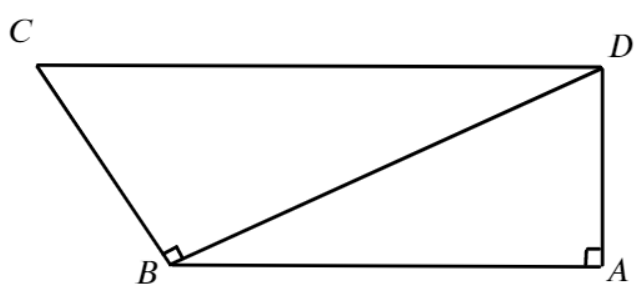
\includegraphics[scale=0.35]{g8-28.png}}
\end{figure}\\
Так как $8^2+15^2=17^2$ и $9^2+12^2=15^2,$ по обратной теореме Пифагора треугольники $BCD$ и $BAD$ являются прямоугольными. Тогда $S_{ABCD}=S_{BCD}+S_{BAD}=\cfrac{1}{2}\cdot8\cdot15+\cfrac{1}{2}\cdot9\cdot12=114.$\\
